
\documentclass{article}
\usepackage{fontenc}
\usepackage[english]{babel}
\usepackage[latin1]{inputenc}
\usepackage{babel}
\usepackage{indentfirst} %auto-indent first paragraphs in sections
\usepackage{verbatim}
\usepackage{url}
\usepackage{fancyhdr} % Required for custom headers
\usepackage{lastpage} % Required to determine the last page for the footer
\usepackage{extramarks} % Required for headers and footers
\usepackage{graphicx} % Required to insert images
\usepackage{subfigure} %for horizontally placed pictures
\usepackage{hyperref} %to make table of contents clickable
\hypersetup{
	colorlinks,
	citecolor=black,
	filecolor=black,
	linkcolor=black,
	urlcolor=black
	}

\usepackage{multirow}

% Margins
\topmargin=-0.45in
\evensidemargin=0in
\oddsidemargin=0in
\textwidth=6.5in
\textheight=9.0in
\headsep=0.25in 
\linespread{1.1} % Line spacing

% Set up the header and footer
\pagestyle{fancy}
\lhead{\myAuthorName} % Top left header
\chead{\myTitle} % Top right header
%\rhead{\myDate}
\rhead{\today}
\lfoot{} % Bottom left footer
\cfoot{} % Bottom center footer
\rfoot{Page\ \thepage\ of\ \pageref{LastPage}} % Bottom right footer
\renewcommand\headrulewidth{0.4pt} % Size of the header rule
\renewcommand\footrulewidth{0.4pt} % Size of the footer rule

\newcommand{\myTitle}{Cluster Merging Algorithms Documentation}
\newcommand{\myAuthorName}{David Caratelli, David Kaleko}
%\newcommand{\myDate}{January, 2013}
%----------------------------------------------------------------------------------------


\title{\myTitle}
\author{\myAuthorName}
\date{\today}


\begin{document}
\maketitle

\newpage

\tableofcontents

\newpage


\section{to-do in this documentation}
\begin{itemize}
\item fill in the missing stuff so far (marked with ``davidc" or ``xxx")
\item fill in the ``other algorithms" section
\item combine this documentation with ``matching" documentation
\item include all of the priority, prohibit algorithms that are not included yet (i've included all merge algorithms, and the prohibit/prioritiy algorithms used in first/second stage merging, but not all prohibit/priority algos that aren't used)
\item appendix on polygons
\end{itemize}

%%%%%%%%%%%%%%%%%%%%%%%%%%%%%%%%%%%%%%%%%%
\section{Overview}
\footnote{As an initial note, this documentation describes cluster merging algorithms as they are coded as of the time this document was$\nu_e$CC written (May 1st, 2015). These algorithms, as described, were used in both MCC4 and MCC5 productions on MicroBooNE.} The output of Fuzzycluster is usually many small clusters. An example of raw Fuzzycluster output on a clean single $\pi^0$ event is shown in \autoref{raw_fuzzy_pi0_fig} and on a single $\nu_e$CC event is shown in \autoref{raw_fuzzy_nue_fig}. In order to be able to reconstruct a meaningful shower object, it is necessary to combine these small clusters together. It is important not to merge clusters that come from different physical particles, as there is no un-merging process downstream. \\\\
\indent Developers have decided that cluster merging is best done in multiple steps, so merging is broken up into ``preliminary" and ``second stage merging". After first stage merging comes track removal (necessary for shower reconstruction), then second stage merging happens only on the remaining shower-like clusters. If necessary, a third stage merging can be implemented as well, but it does not exist yet.

\begin{figure}[h!]
\begin{center}
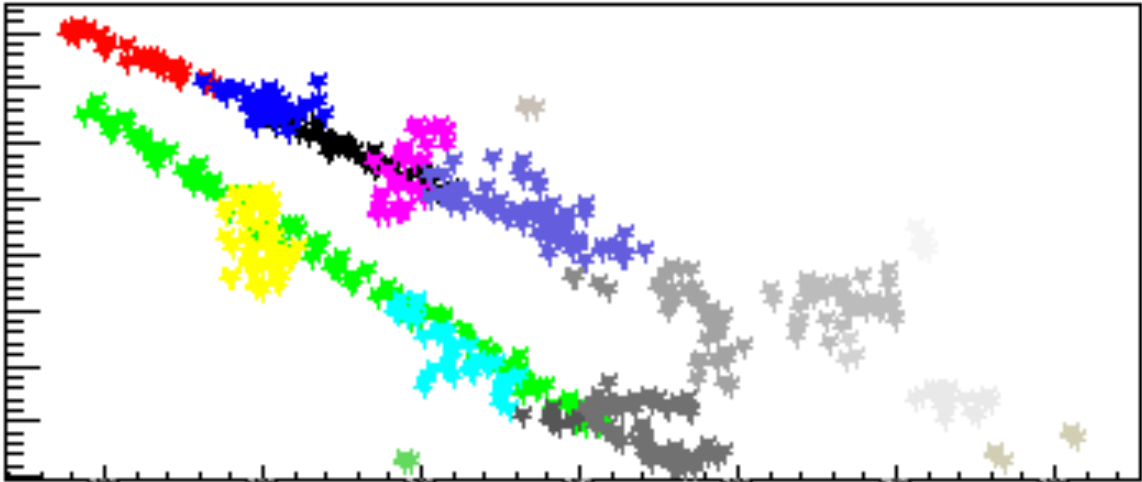
\includegraphics[width=110mm]{Figures/raw_fuzzy_pi0.png}
\end{center}
\caption{\textit{A very clean $\pi^0$ event, Fuzzycluster output from one plane. The y- axis is time, the x- axis is wire number. Each different color corresponds to a different cluster.}}
\label{raw_fuzzy_pi0_fig}
\end{figure}

\begin{figure}[h!]
\begin{center}
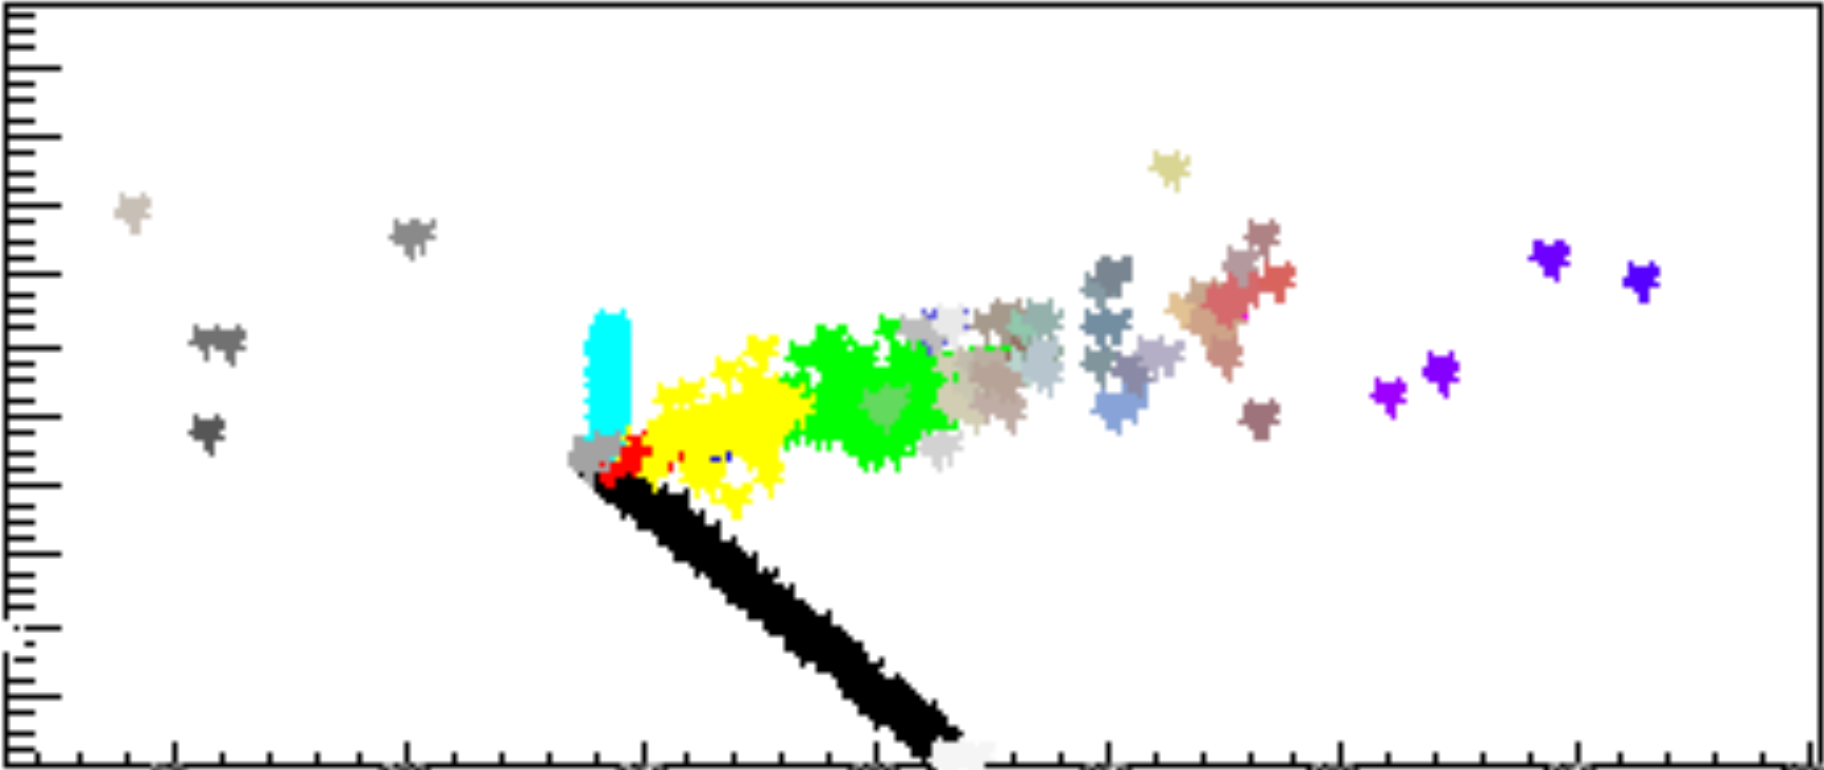
\includegraphics[width=110mm]{Figures/raw_fuzzy_nue.png}
\end{center}
\caption{\textit{A very clean $\nu_e$CC event, Fuzzycluster output from one plane. The y- axis is time, the x- axis is wire number. Each different color corresponds to a different cluster.}}
\label{raw_fuzzy_nue_fig}
\end{figure}

\subsection{Preliminary (First-Stage) Merging}
The input of preliminary merging are clusters directly output by Fuzzycluster. A screenshot of the Fuzzycluster output of a very clean $\pi^0$ event is shown in \autoref{raw_fuzzy_pi0_fig} and on a single $\nu_e$CC event is shown in \autoref{raw_fuzzy_nue_fig}. The purpose of preliminary merging is two-fold.
\begin{itemize}
\item Showers often have a small, track-like cluster at their start. This needs to be merged with the rest of the shower-like clusters it leads in to, so it won't get removed in the track removal stage.
	\begin{enumerate}
	\item This is especially important because this cluster is generally where the important $\frac{dE}{dx}$ information comes from for showers.
	\end{enumerate}
\item ``Obvious" merging of clusters (that are clearly from the same shower) is done here. Note, if it is not obvious, the clusters are not merged, and that responsibility is passed on to second-stage merging. \textit{There is no un-merging.}
\end{itemize}
Preliminary merging is run with the ``MergeTillConverge" flag set to true. The different algorithms used in preliminary merging and their purposes are described in \textbf{\autoref{sec:PrelimMerging}}. To understand these descriptions (for example, what a ``prohibit" algorithm is, or a ``priority algorithm" is, or an ``algo array" is, or what ``MergeTillConverge" is), the reader may have to refer to documentation on the merging framework put together by Kazu (docDB reference here). A screenshot of the same $\pi^0$ event as shown in \autoref{raw_fuzzy_pi0_fig} after preliminary merging is shown in \autoref{prelim_fuzzy_pi0_fig}. A screenshot of the same $\nu_e$CC event as shown in \autoref{raw_fuzzy_nue_fig} after preliminary merging is shown in \autoref{prelim_fuzzy_nue_fig}.


\begin{figure}[h!]
\begin{center}
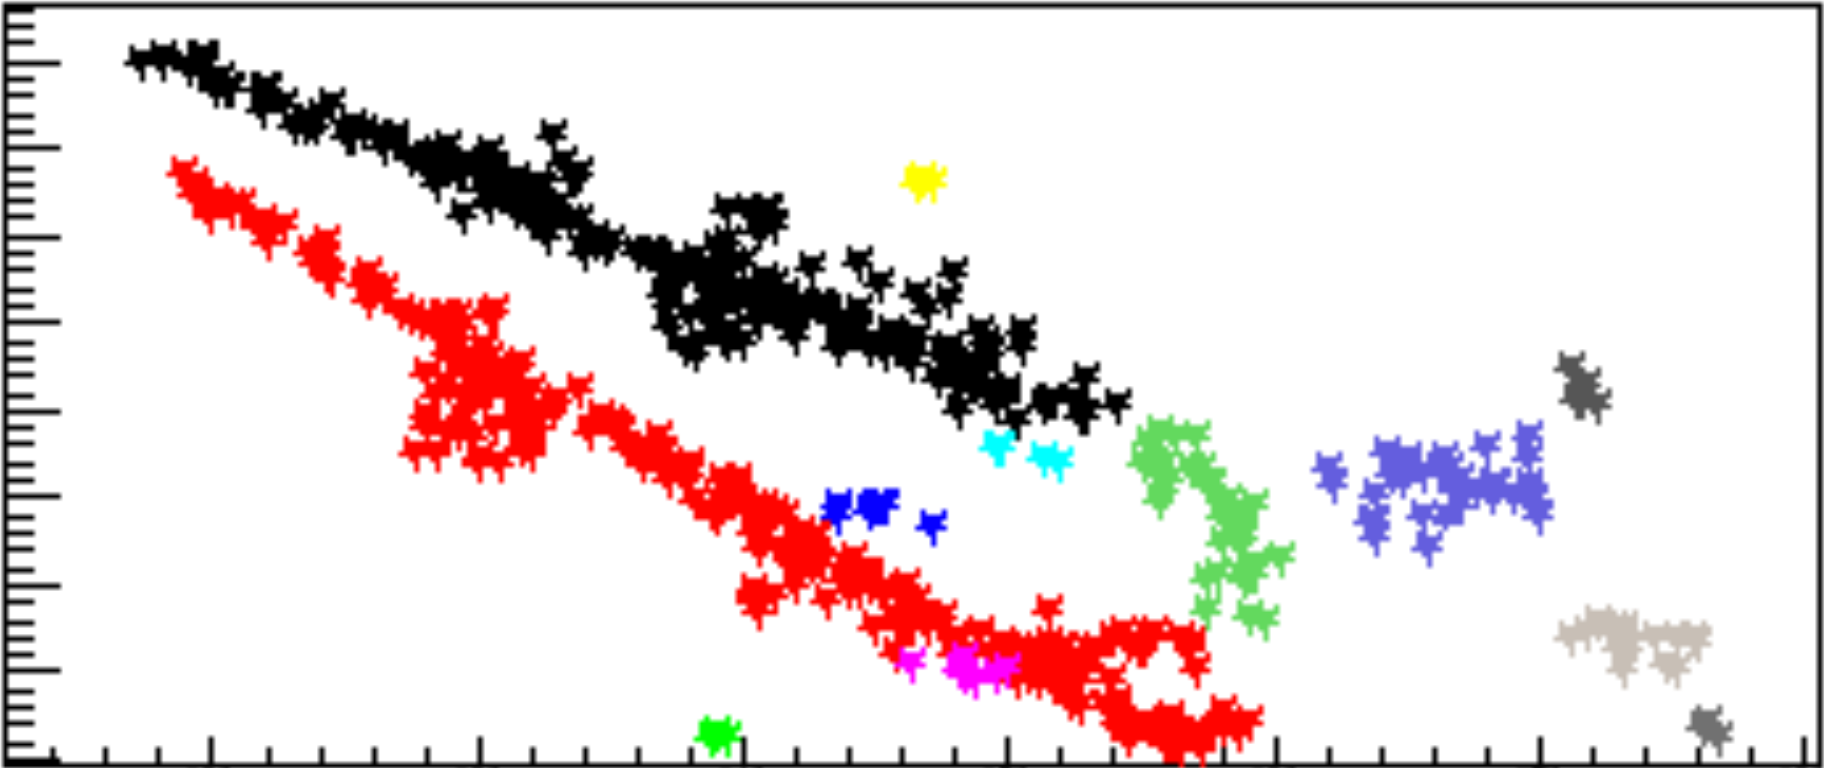
\includegraphics[width=110mm]{Figures/prelim_fuzzy_pi0.png}
\end{center}
\caption{\textit{The same $\pi^0$ event as shown in \autoref{raw_fuzzy_pi0_fig} after preliminary merging. The color of clusters in this plot are unrelated to the colors of clusters in \autoref{raw_fuzzy_pi0_fig}.}}
\label{prelim_fuzzy_pi0_fig}
\end{figure}

\begin{figure}[h!]
\begin{center}
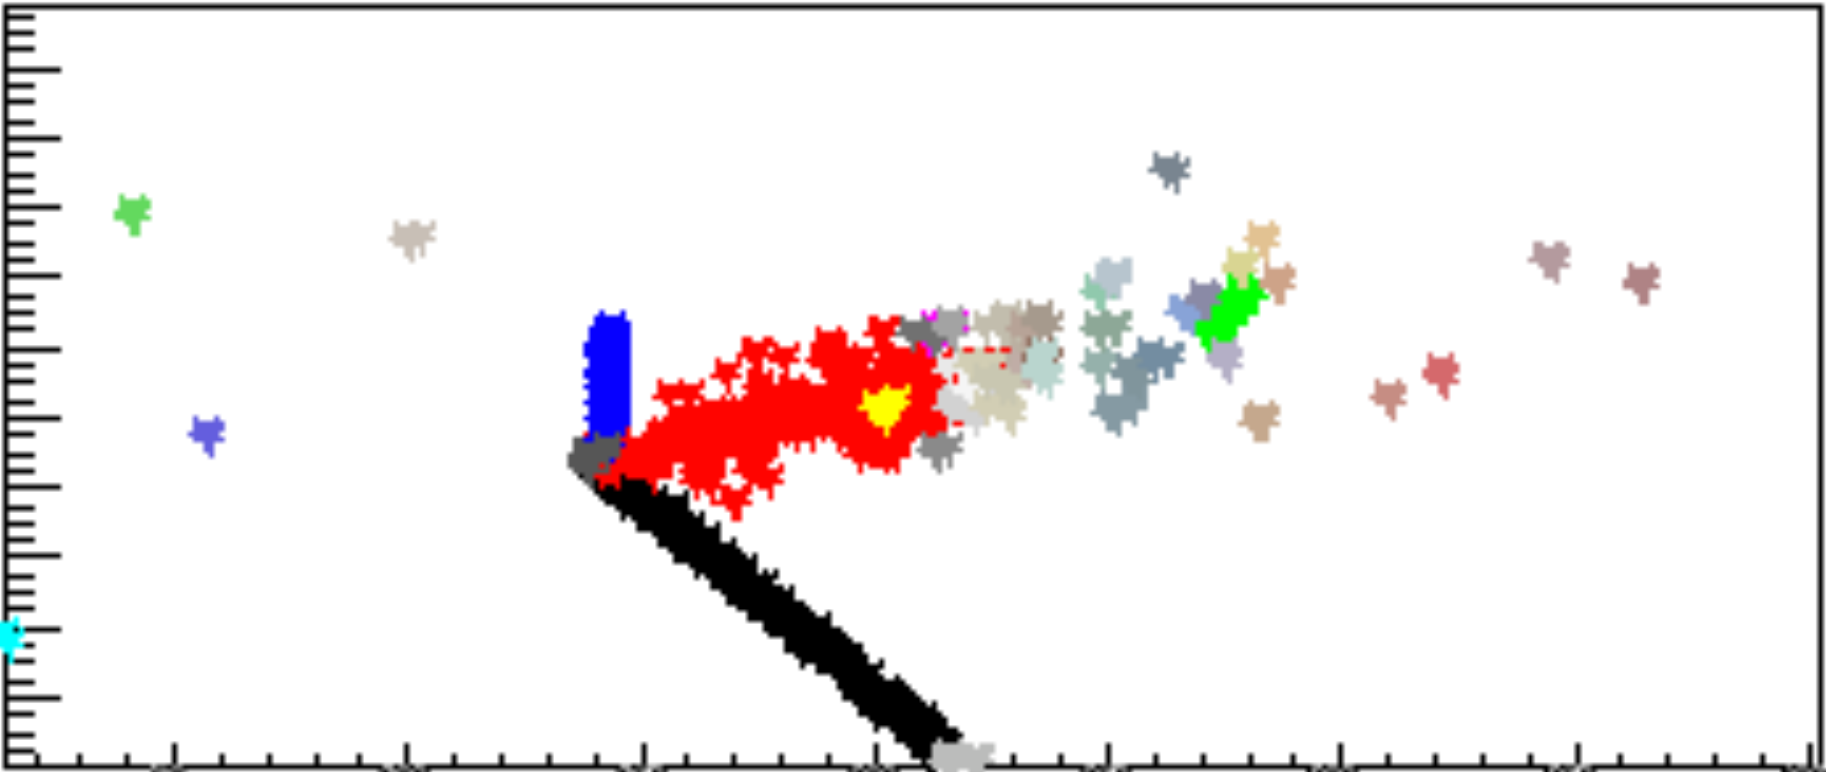
\includegraphics[width=110mm]{Figures/prelim_fuzzy_nue.png}
\end{center}
\caption{\textit{The same $\nu_e$CC event as shown in \autoref{raw_fuzzy_nue_fig} after preliminary merging. The color of clusters in this plot are unrelated to the colors of clusters in \autoref{raw_fuzzy_nue_fig}.}}
\label{prelim_fuzzy_nue_fig}
\end{figure}

\subsection{Second Stage Merging}
The input of second stage merging are clusters already merged by preliminary clusters, excluding all ``track-like" clusters that remained after preliminary merging. The definition of ``track-like" clusters is described in \textbf{\autoref{sec:CBAlgoTrackSeparate}}. The output of second stage merging are clusters that are used as input for shower reconstruction.\\\\
Second stage merging is run with the ``MergeTillConverge" flag set to true. The different algorithms used in second stage merging and their purposes are described in \textbf{\autoref{sec:SecondMerging}}. A screenshot of the same $\pi^0$ event as shown in \autoref{raw_fuzzy_pi0_fig} and \autoref{prelim_fuzzy_pi0_fig} after second merging is shown in \autoref{second_fuzzy_pi0_fig}.  A screenshot of the same $\nu_e$CC event as shown in \autoref{raw_fuzzy_nue_fig} and \autoref{prelim_fuzzy_pi0_fig} after second merging is shown in \autoref{second_fuzzy_nue_fig}.



\begin{figure}[h!]
\begin{center}
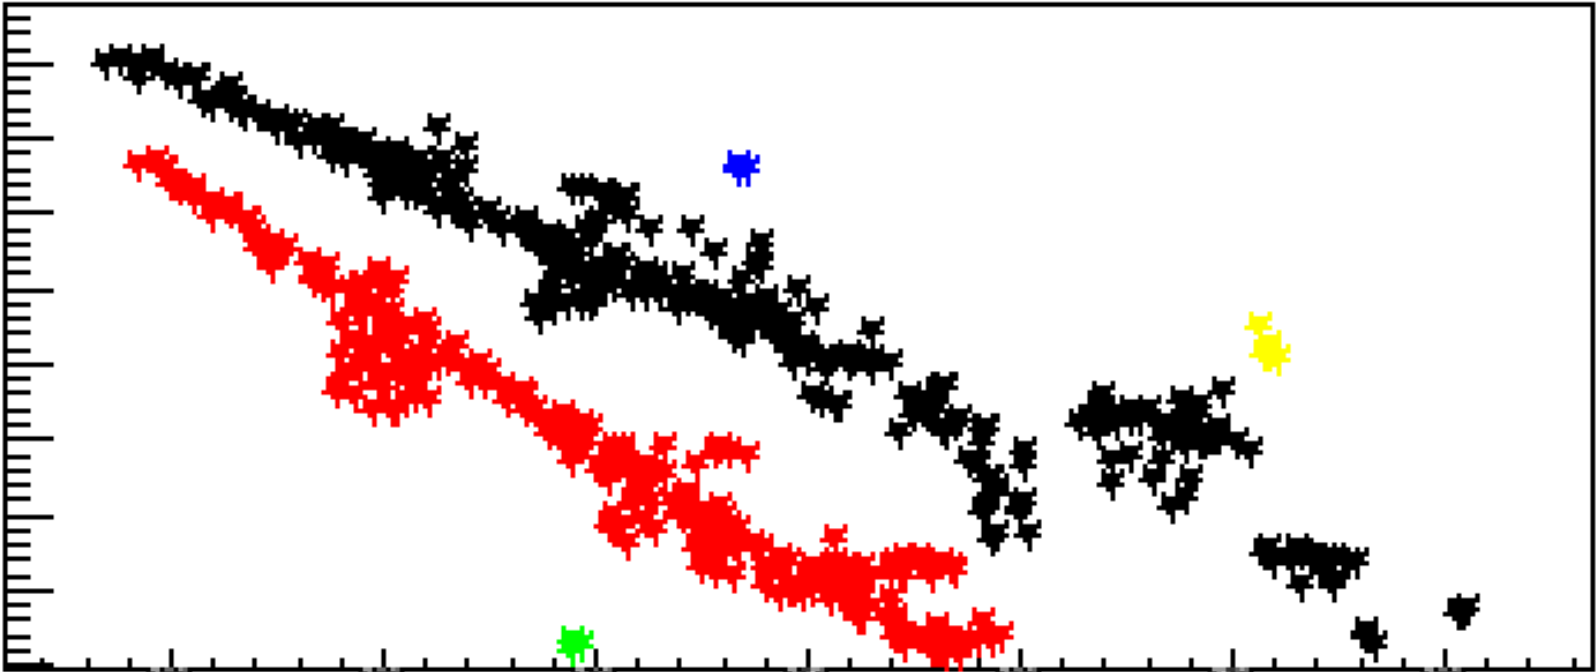
\includegraphics[width=110mm]{Figures/second_fuzzy_pi0.png}
\end{center}
\caption{\textit{The same $\pi^0$ event as shown in \autoref{raw_fuzzy_pi0_fig} and \autoref{prelim_fuzzy_pi0_fig}, now after second stage merging. The color of clusters in this plot are unrelated to the colors of clusters in \autoref{raw_fuzzy_pi0_fig} and \autoref{prelim_fuzzy_pi0_fig}.}}
\label{second_fuzzy_pi0_fig}
\end{figure}

\begin{figure}[h!]
\begin{center}
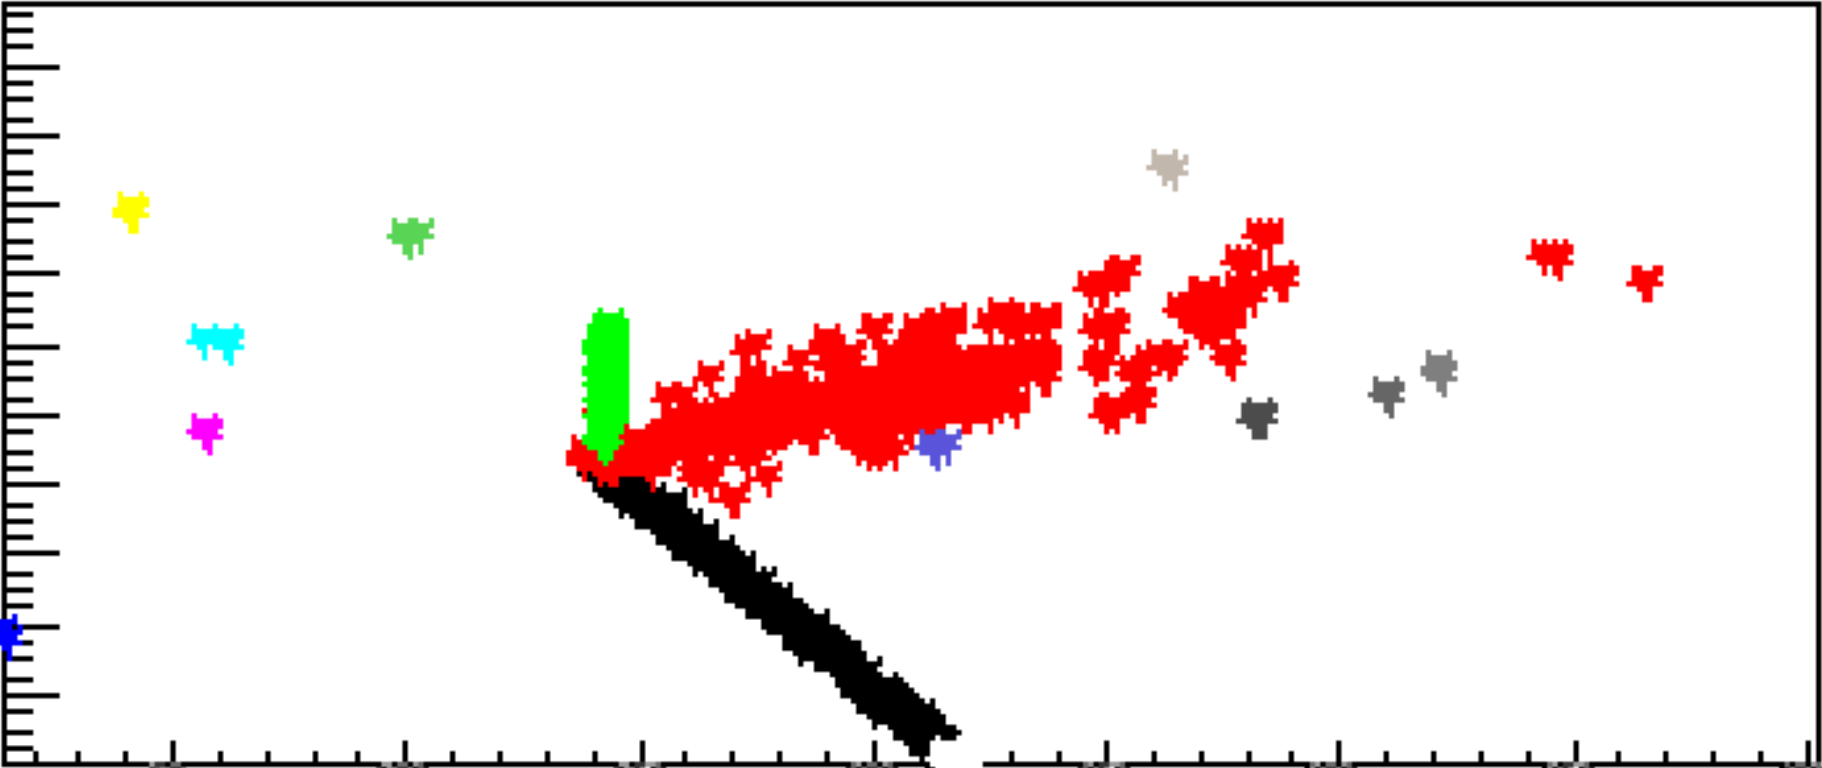
\includegraphics[width=110mm]{Figures/second_fuzzy_nue.png}
\end{center}
\caption{\textit{The same $\nu_e$CC event as shown in \autoref{raw_fuzzy_nue_fig} and \autoref{prelim_fuzzy_nue_fig}, now after second stage merging. The color of clusters in this plot are unrelated to the colors of clusters in \autoref{raw_fuzzy_nue_fig} and \autoref{prelim_fuzzy_nue_fig}.}}
\label{second_fuzzy_nue_fig}
\end{figure}

%%%%%%%%%%%%%%%%%%%%%%%%%%%%%%%%%%%%%%%%%%
\section{Quick Reference: List Of Algorithms}
The following is a list of all merging algorithms (in alphabetical order) as of the time this document was produced, along with a clickable link to the section of this document that describes that algorithm.
\begin{enumerate}
\item CBAlgoAngleAlign \textbf{(\autoref{sec:CBAlgoAngleAlign})}
\item CBAlgoAngleCompat \textbf{(\autoref{sec:CBAlgoAngleCompat})}
\item CBAlgoAngleIncompat \textbf{(\autoref{sec:CBAlgoAngleIncompat})}
\item CBAlgoAngleSeparate \textbf{(\autoref{sec:CBAlgoAngleSeparate})}
\item CBAlgoArray \textbf{(\autoref{sec:CBAlgoArray})}
\item CBAlgoCenterOfMass \textbf{(\autoref{sec:CBAlgoCenterOfMass})}
\item CBAlgoCenterOfMassSmall \textbf{(\autoref{sec:CBAlgoCenterOfMassSmall})}
\item CBAlgoFake \textbf{(\autoref{sec:CBAlgoFake})}
\item CBAlgoMergeAll \textbf{(\autoref{sec:CBAlgoMergeAll})}
\item CBAlgoMergeTinyWithBig \textbf{(\autoref{sec:CBAlgoMergeTinyWithBig})}
\item CBAlgoOutOfConeSeparate \textbf{(\autoref{sec:CBAlgoOutOfConeSeparate})}
\item CBAlgoPolyContain \textbf{(\autoref{sec:CBAlgoPolyContain})}
\item CBAlgoPolyHitOverlap \textbf{(\autoref{sec:CBAlgoPolyHitOverlap})}
\item CBAlgoPolyOverlap \textbf{(\autoref{sec:CBAlgoPolyOverlap})}
\item CBAlgoPolyShortestDist \textbf{(\autoref{sec:CBAlgoPolyShortestDist})}
\item CBAlgoProhibitAllTracks \textbf{(\autoref{sec:CBAlgoProhibitAllTracks})}
\item CBAlgoProhibitBigClusters \textbf{(\autoref{sec:CBAlgoProhibitBigClusters})}
\item CBAlgoShortestDist \textbf{(\autoref{sec:CBAlgoShortestDist})}
\item CBAlgoStartInCone \textbf{(\autoref{sec:CBAlgoStartInCone})}
\item CBAlgoStartInPoly \textbf{(\autoref{sec:CBAlgoStartInPoly})}
\item CBAlgoStartNearEnd \textbf{(\autoref{sec:CBAlgoStartNearEnd})}
\item CBAlgoStartTrack \textbf{(\autoref{sec:CBAlgoStartTrack})}
\item CBAlgoTrackSeparate \textbf{(\autoref{sec:CBAlgoTrackSeparate})}
\end{enumerate}

%%%%%%%%%%%%%%%%%%%%%%%%%%%%%%%%%%%%%%%%%%
\newpage
\section{Algorithms Used In Preliminary (First-Stage) Merging}\label{sec:PrelimMerging}

\begin{figure}[h!]
\begin{center}
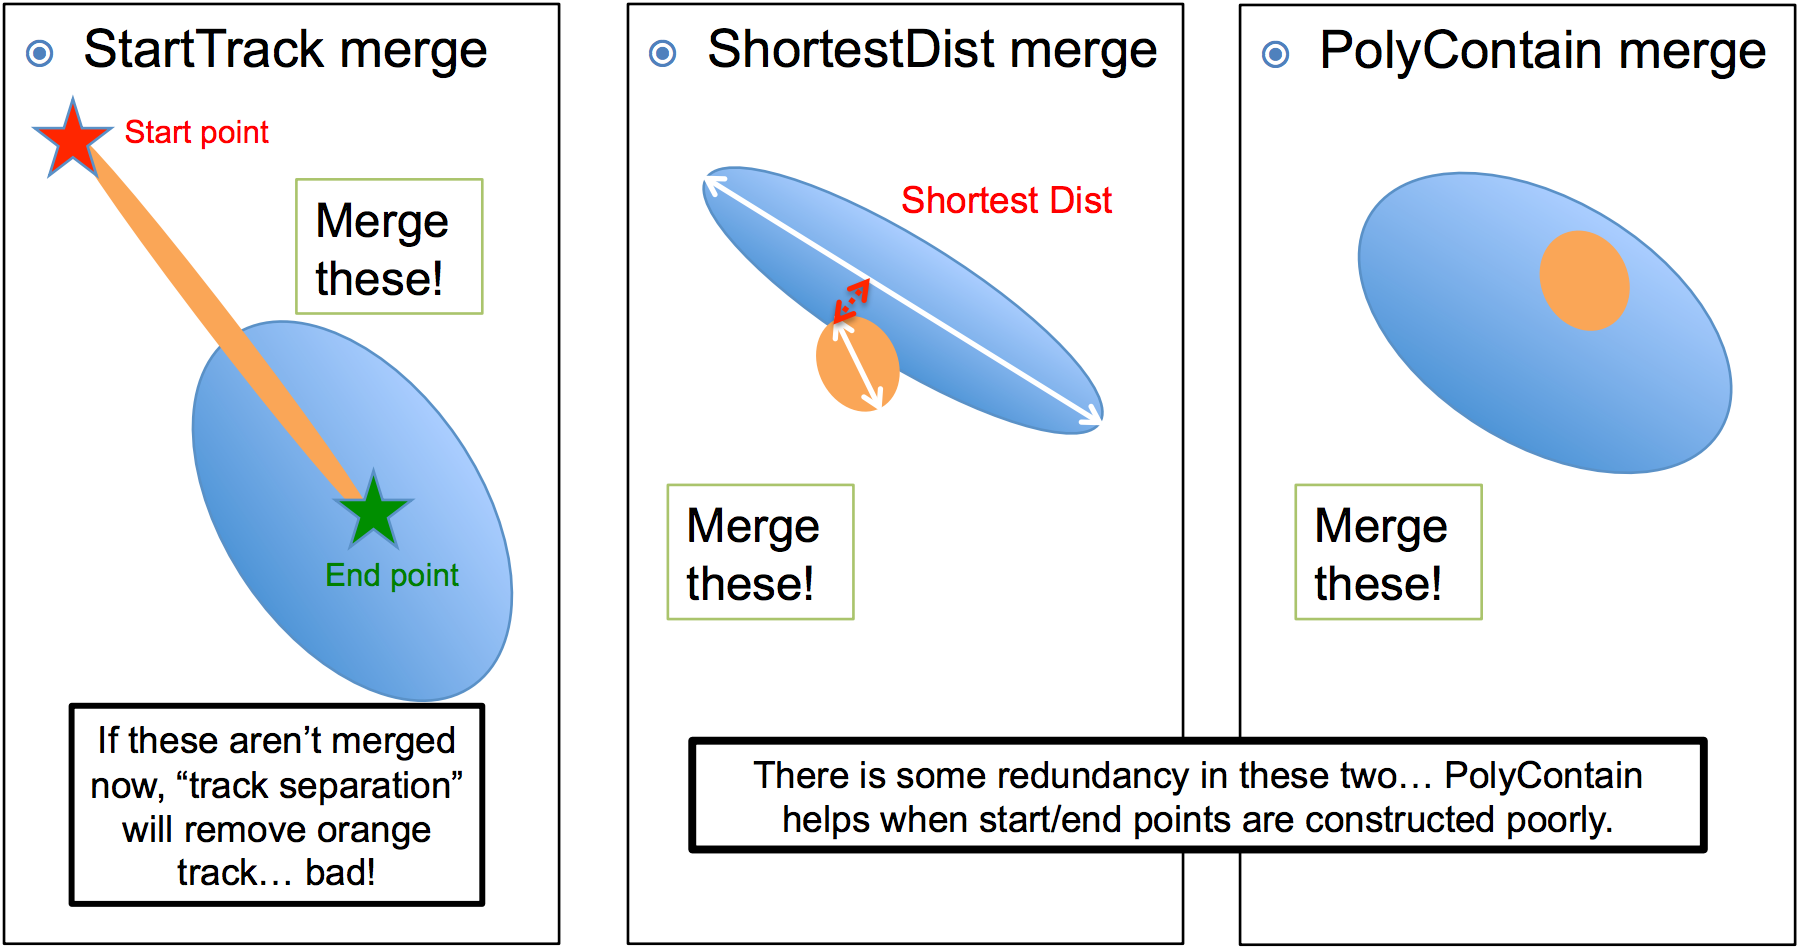
\includegraphics[width=150mm]{Figures/prelim_merge_algos.png}
\end{center}
\caption{\textit{Diagrams describing the three preliminary merge algorithms used. Each blob (blue, or orange) represents a different cluster. For more information on the individual algorithms, see their corresponding subsections within this section.}}
\label{prelim_merge_algos_fig}
\end{figure}

\begin{figure}[h!]
\begin{center}
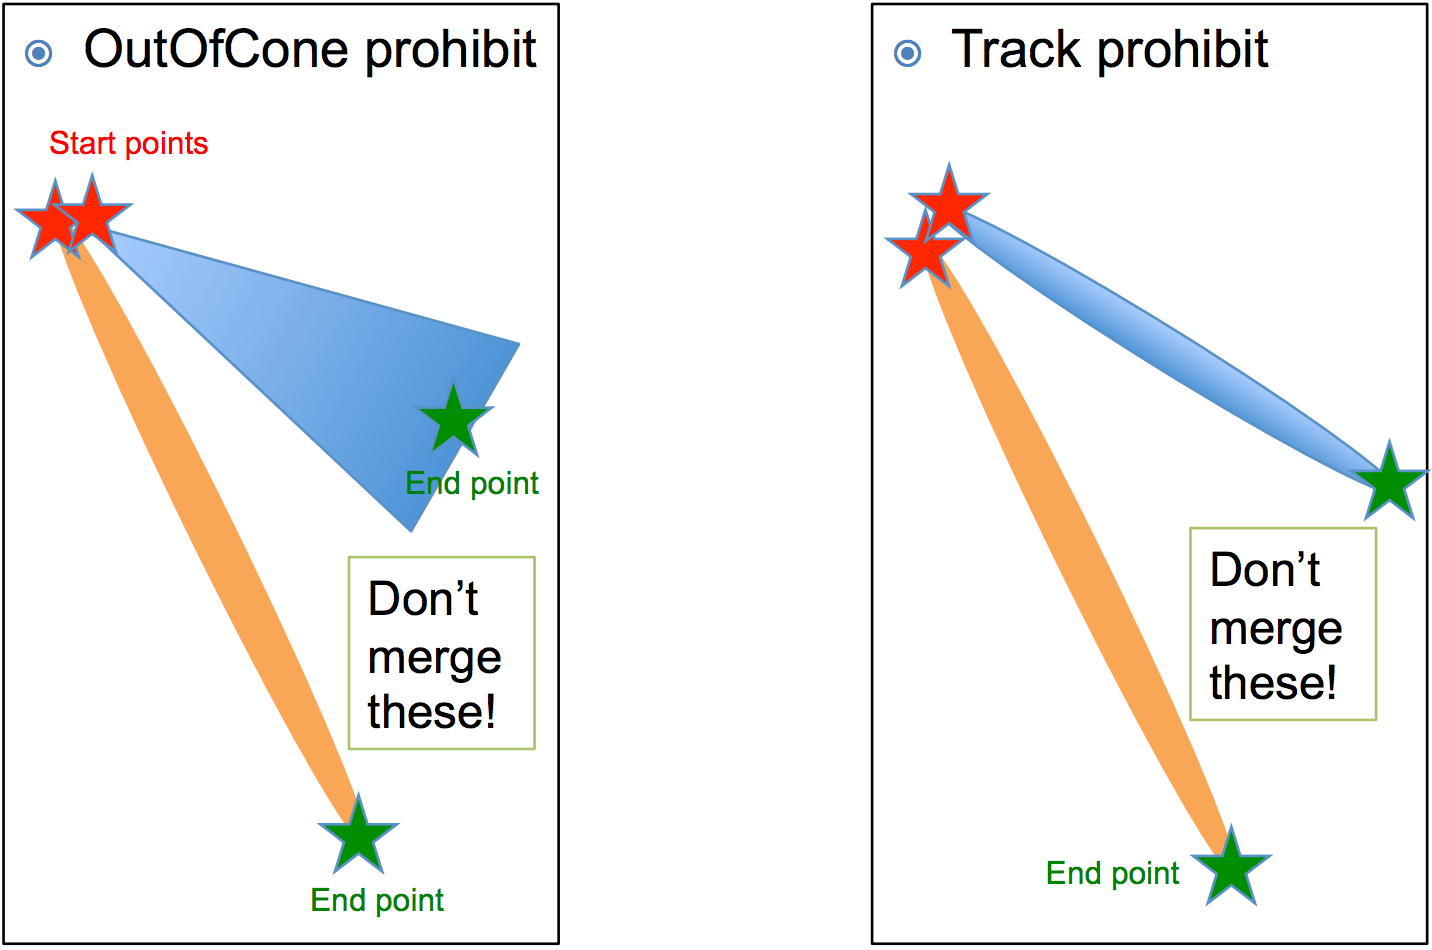
\includegraphics[width=110mm]{Figures/prelim_prohibit_algos.png}
\end{center}
\caption{\textit{Diagrams describing the three preliminary prohibit algorithms used. Each blob (blue, or orange) represents
a different cluster. For more information on the individual algorithms, see their corresponding subsections within this 
section.}}
\label{prelim_prohibit_algos_fig}
\end{figure}


\subsection{CBAlgoTrackSeparate}\label{sec:CBAlgoTrackSeparate}
This algorithm is a prohibit algorithm. Its purpose is to prevent the merging of two clusters in the case that both
clusters qualify as ``track-like". If the ``UseEP" flag is set to true (which it is in the instance of this algorithm 
used for preliminary merging), then a cluster is considered ``track-like" if its principal eigenvalue is greater than 
some cutoff value. This cutoff value is set to 0.99000.


\subsection{CBAlgoOutOfConeSeparate}\label{sec:CBAlgoOutOfConeSeparate}
This algorithm is a prohibit algorithm. Its purpose is to prevent the merging of two clusters in the case that the angle
between the direction of a cluster (end-start) and the line connecting the cluster's start point and the start point of 
a second cluster is too large. The first cluster needs to be a "good" and "large" cluster to be considered by this 
algorithm.\\
The angle cut becomes tighter as the separation between the two cluster's start points increases.

The maximum angle separation is set to 20 degrees for preliminary merging.\\
SetMinLength(15.);\\
SetMinHits(20);\\
SetStartAngleFalloff(2800); // in cm\^2 \\
    
\begin{figure}[h!]
\begin{center}
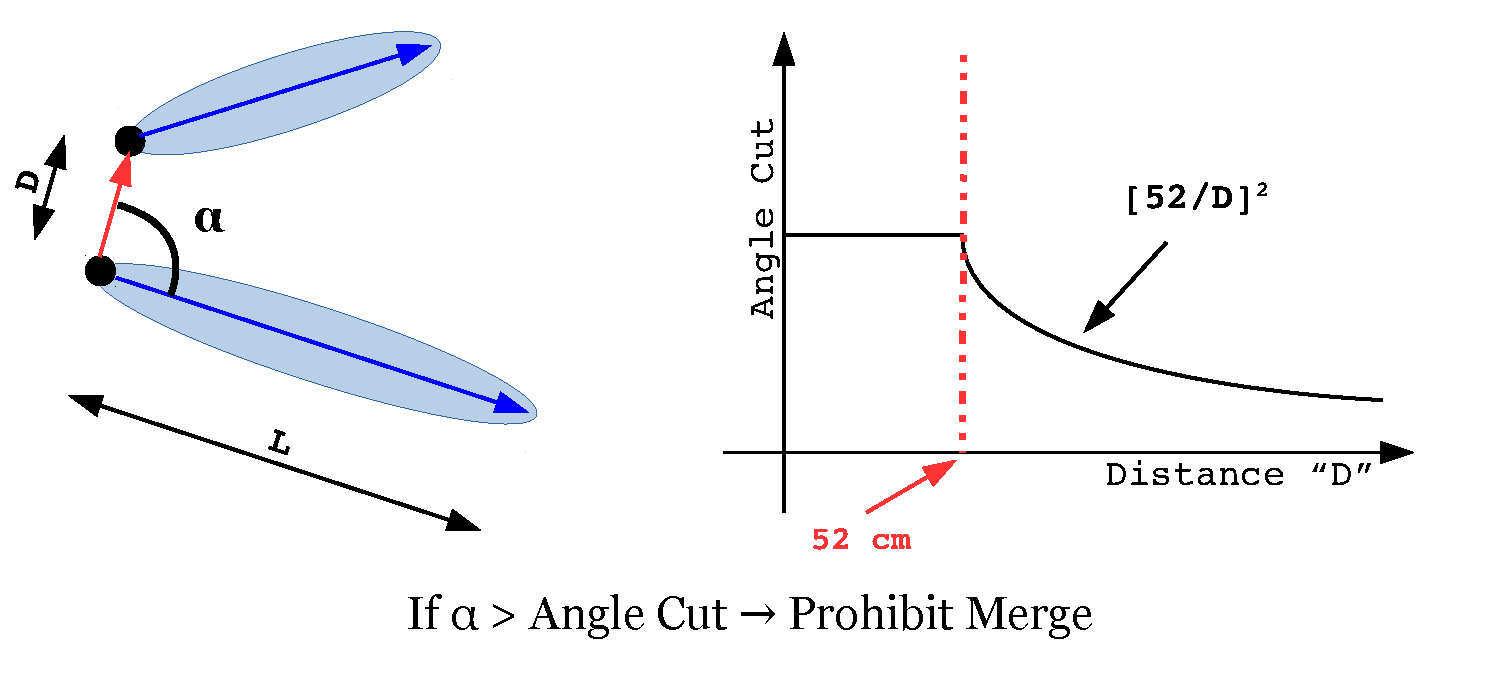
\includegraphics[width=150mm]{Figures/CBAlgoOutOfConeSeparate.pdf}
\end{center}
\caption{\textit{Diagram demonstrating how CBAlgoOutOfConeSeparate works. A cut is placed on the maximum allowed
angle between a cluster's direction and the line connecting that cluster's start point and the start point of
the second cluster under consideration. As the two clusters become more separated, the constraint on this angle
becomes tighter.}}
\label{fig:CBAlgoOutOfConeSeparate}
\end{figure}
    
    
\subsection{CBAlgoShortestDist}\label{sec:CBAlgoShortestDist}
This algorithm is a merging algorithm. It takes in the start, and end points of each of the two input clusters and 
computes the distance-squared (to save computing time in taking a square root) between each of the four pairs of points 
(start1-to-start2, start1-to-end2, end1-to-start2, end1-to-end2). If the minimum of these four distances is less than
a cutoff value, the two clusters are merged.\\\\
For preliminary merging, the minimum number of hits for each cluster to be considered is set to 10 and the shortest 
distance-squared value is set to 5 cm.

\subsection{CBAlgoStartTrack}\label{sec:CBAlgoStartTrack}
This algorithm is a merging algorithm. Its purpose is to merge track-like clusters if they are leading into a shower-like
cluster. This is because Fuzzycluster often creates short, track-like clusters at the beginning of showers. This merging 
is particularly important because the leading track-like cluster contains most of the $\frac{dE}{dx}$ information that is
important for identifying the particle that created this shower.\\\\
This algorithm first identifies if one of the clusters is track-like by requiring that cluster's principal eigenvalue be
greater than some cutoff, currently set to 0.99000. Then, it identifies if the other cluster is shower-like by asking that 
the width of the cluster is greater than some cutoff, currently set to 1mm, as well as asking that the opening angle of 
the cluster is greater than some cutoff, currently set to 0.15, as well as asking that the principal eigenvalue is less 
than some cutoff, currently set to 0.99000. Then, it asks that the endpoint of the track-like cluster is within the polygon
outlining the shower-like cluster. If all of these conditions are met, the two clusters are merged.

\subsection{CBAlgoPolyContain}\label{sec:CBAlgoPolyContain}
This algorithm is a merging algorithm. Its purpose is to merge two clusters if the polygon object outlining one cluster
is completely contained with the polygon object outlining the other cluster.

%%%%%%%%%%%%%%%%%%%%%%%%%%%%%%%%%%%%%%%%%%
\newpage
\section{Algorithms Used In Second-Stage Merging} \label{sec:SecondMerging}
\begin{figure}[h!]
\begin{center}
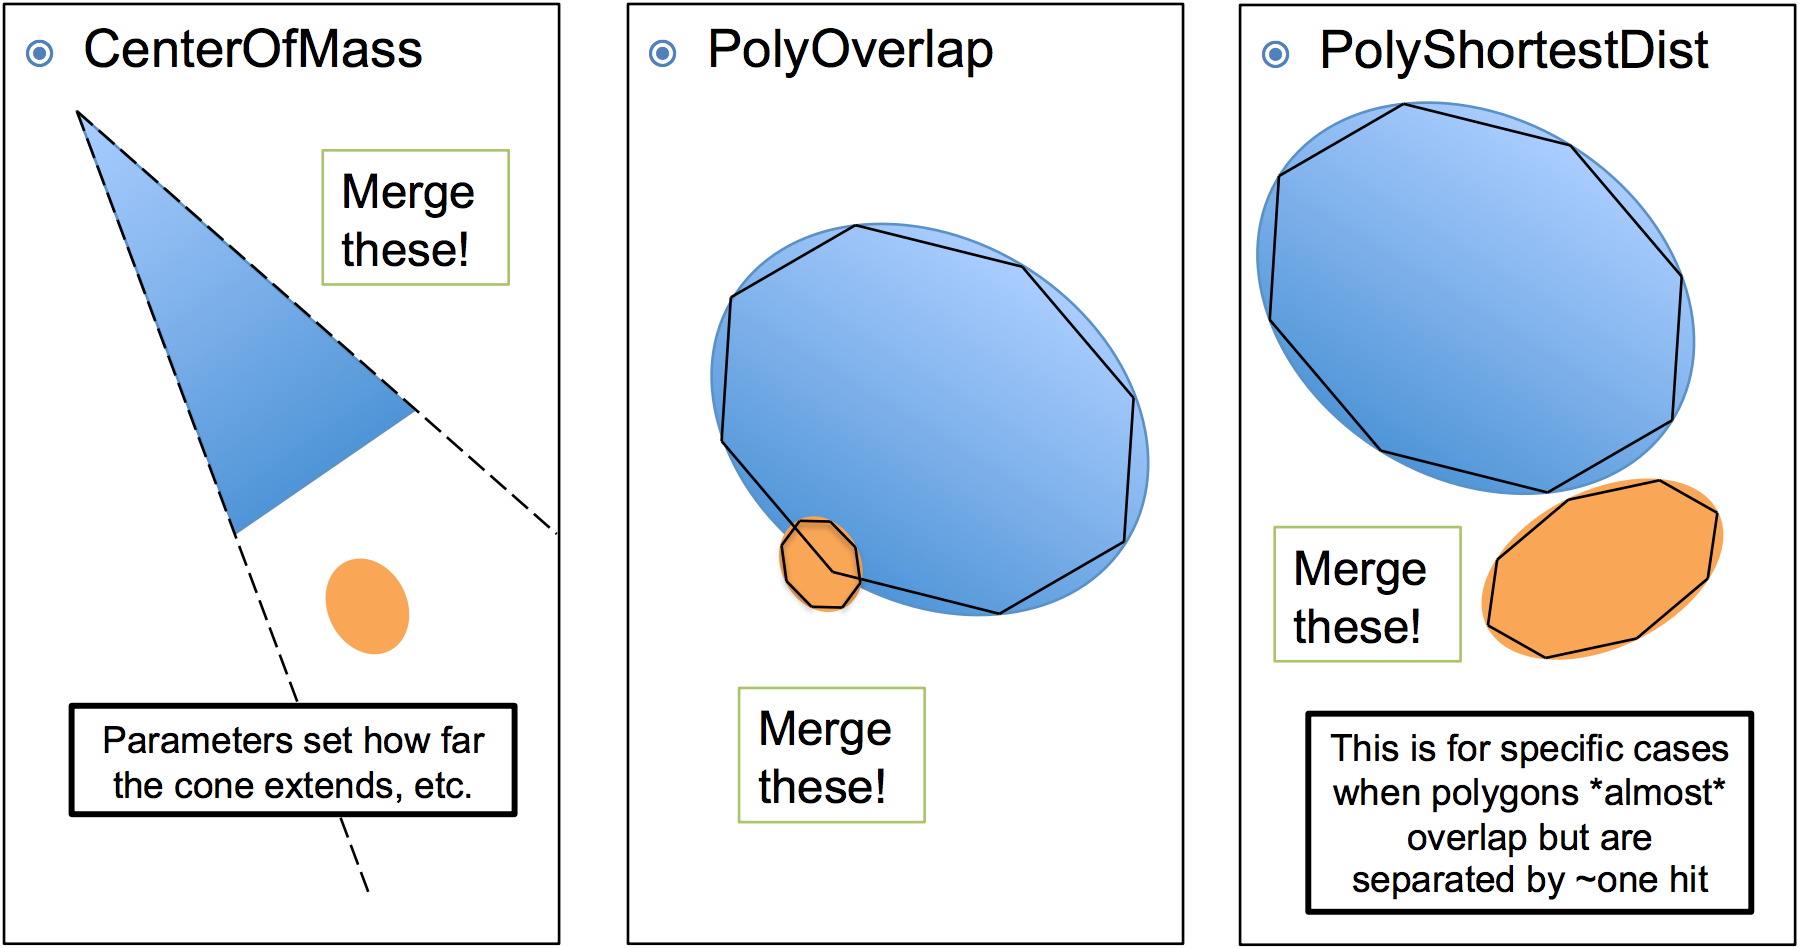
\includegraphics[width=140mm]{Figures/second_merge_algos.png}
\end{center}
\caption{\textit{Diagrams describing the three secondinary merge algorithms used. Each blob (blue, or orange) represents 
a different cluster. For more information on the individual algorithms, see their corresponding subsections within this 
section.}}
\label{second_merge_algos_fig}
\end{figure}

\begin{figure}[h!]
\begin{center}
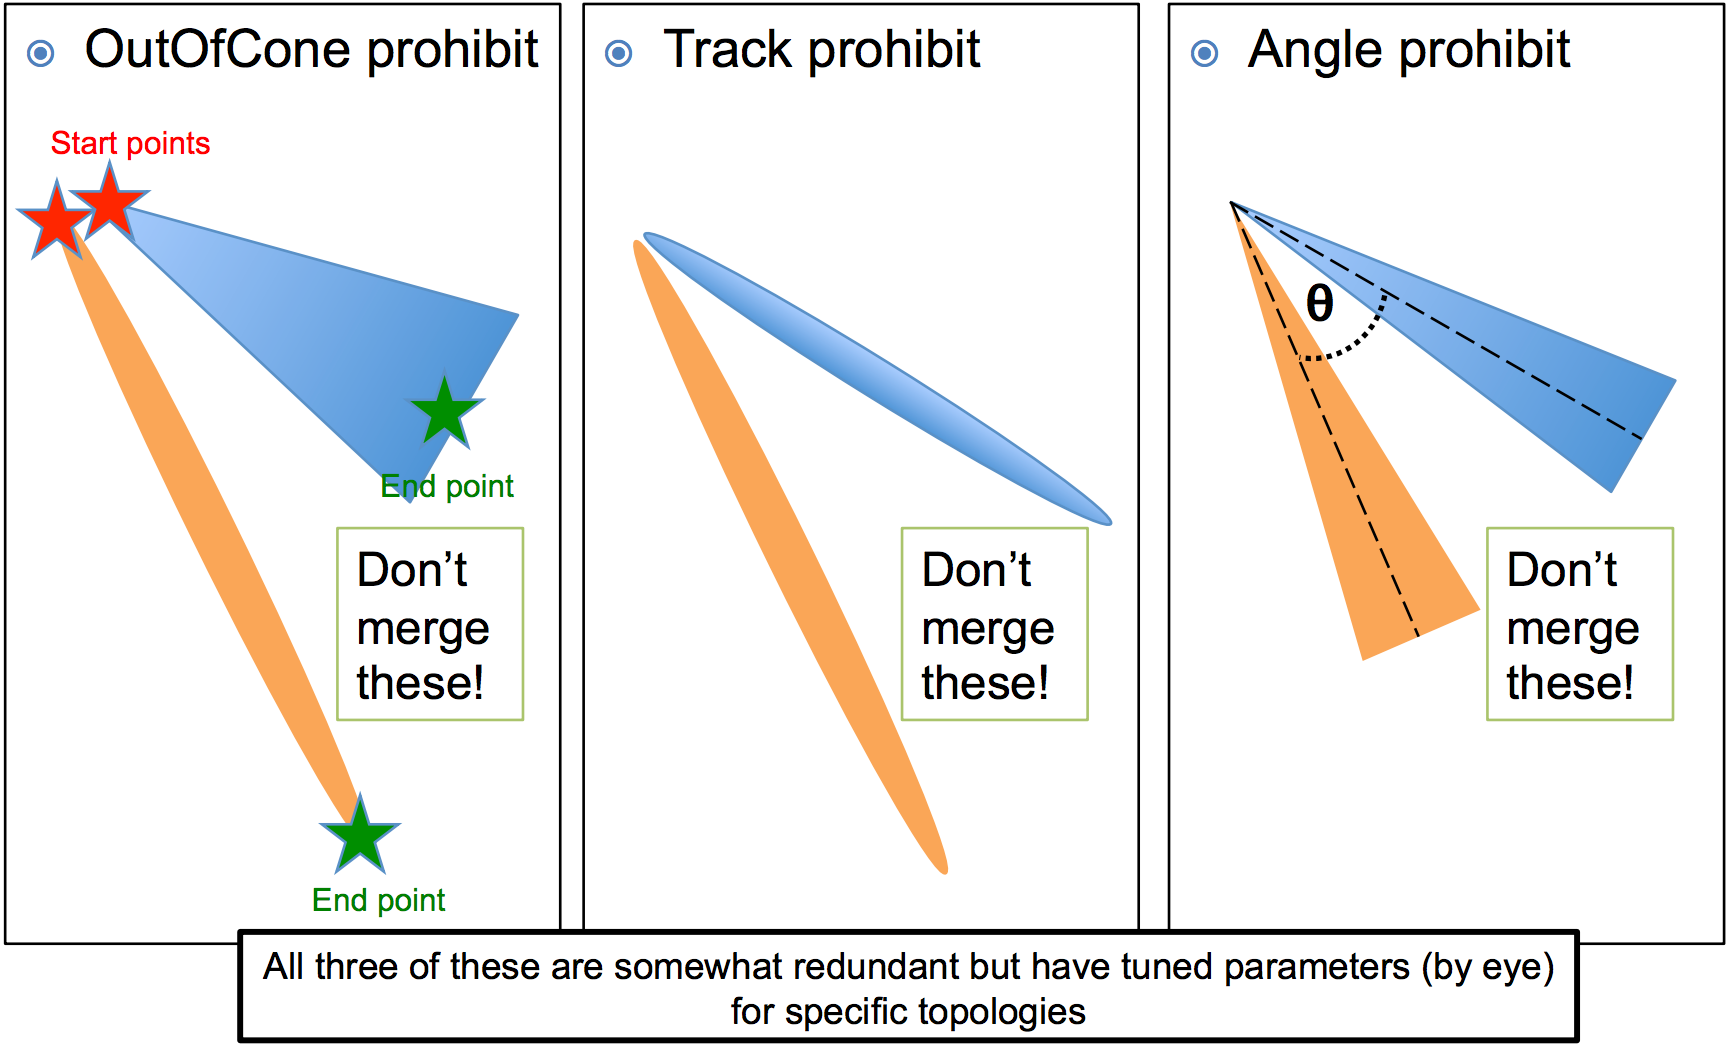
\includegraphics[width=140mm]{Figures/second_prohibit_algos.png}
\end{center}
\caption{\textit{Diagrams describing the three secondinary prohibit algorithms used. Each blob (blue, or orange)
represents a different cluster. For more information on the individual algorithms, see their corresponding 
subsections within this section.}}
\label{second_prohibit_algos_fig}
\end{figure}


\subsection{CPAlgoIgnoreTracks}\label{sec:CPAlgoIgnoreTracks}
This is a priority algorithm that identifies all clusters remaining after preliminary merging that are track-like, and
prevents these clusters from being considered by second stage merging algorithms. This algorithm decides if a cluster is
track-like by requiring the clusters' modified hit density is less than some cutoff (1.4), or multi-hit-wires is less 
than some cutoff (3.5), or log(1-principal eigenvalue) is less than some cutoff (-6).

\subsection{CBAlgoTrackSeparate}
This is a prohibit algorithm, and is re-used second stage merging exactly as is described in the preliminary merge section,
\autoref{sec:CBAlgoTrackSeparate}.

\subsection{CBAlgoOutOfConeSeparate}
This is a prohibit algorithm, and is re-used second stage merging exactly as is described in the preliminary merge section,
\autoref{sec:CBAlgoOutOfConeSeparate}.

\subsection{CBAlgoAngleIncompat}\label{sec:CBAlgoAngleIncompat}
This is a prohibit algorithm which prohibits two clusters from being merged if they are both reasonably large clusters and 
the angle difference between each cluster's 2d angle is greater than some cutoff. Clusters are ``reasonably large" if they
each have above a certain cutoff number of hits (50), and they both have length larger than some cutoff value (20cm). This
algorithm has a flag to allow for backwards-reconstructed clusters (since the 2d angle depends on the cluster's start and
end point positions), and this flag is set to true for second stage merging. This algorithm also has an option to have a 
varying cutoff value for the angle difference based on the opening angles of each cluster. This flag is set to false for 
second stage merging, so a flat cutoff value of 2d angle difference is used (10 degrees).

\subsection{CBAlgoCenterOfMass}\label{sec:CBAlgoCenterOfMass}
This is a merging algorithm designed mainly for merging small clusters into larger ones.\\
A small cluster's Center Of Mass (COM) is calculated as the weighted average (Wire [cm], Time [cm]) of all hits, weighted
by charge. In order to allow merging, the COM needs to be found either:\\
1) inside the large cluster's polygon.\\
2) inside a cone defined by the large cluster's direction and opening angle\\
3) next to the segment connecting the large cluster's start and end point.\\
One, two or all three of these conditions can be used to determine if merging should proceed.\\
\\
Configuration used in 2nd stage merging:\\
if any of the conditions listed above are met merging proceeds.\\
SetMaxHitsSmallClus(10) (set number of hits that define a small cluster)\\
SetMinHitsBigClus(40) (set number of hits that define a big cluster)\\
SetMaxDistance(20) (max. square distance between COM and start-end direction of large cluster)\\
SetLengthReach(3) (spatial extent of cone for large cluster. This factor is the factor multiplying
the length of the cluster and defines the length of the cone)\\
UseCOMInPoly(True)\\
UseCOMInCone(True)\\
UseCOMNearClus(True)\\
\begin{figure}[h!]
\begin{center}
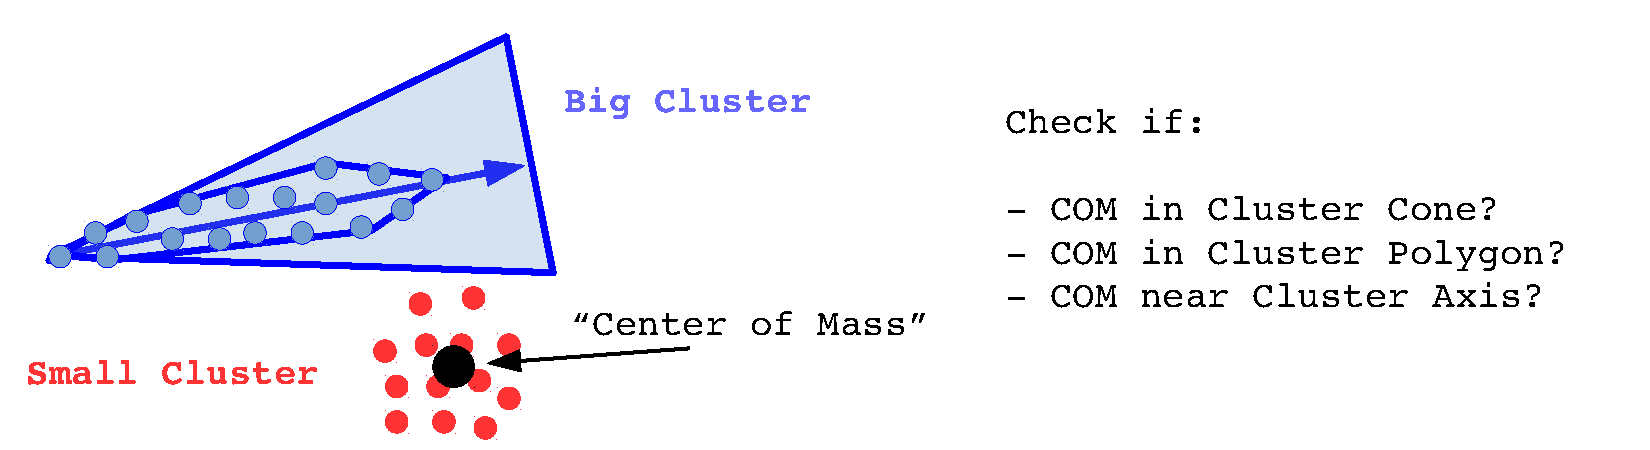
\includegraphics[width=150mm]{Figures/CBAlgoCenterOfMass.pdf}
\end{center}
\caption{\textit{Diagrams describing how CBAlgoCenterOfMass works. A large cluster is compared to a small one. 
Check if the COM is either 1) inside the large cluster's polygon. 2) inside a cone defined by the
long cluster's direction and opening angle. 3) near the line connecting the large cluster's start and end point.
Which of these three conditions are met can be set when the algorithm is initialized.}}
\label{fig:CBAlgoCenterOfMass}
\end{figure}

\subsection{CBAlgoPolyOverlap}\label{sec:CBAlgoPolyOverlap}
This is a merging algorithm, designed to merge two clusters together if a fraction of their polygon's overlapping area is 
greater than some cutoff. The cutoff used in second stage merging is 0, so any overlap will merge the clusters. This 
algorithm also requires that both clusters have greater than some cutoff number of hits (0 for second stage merging).

\subsection{CBAlgoPolyShortestDist}\label{sec:CBAlgoPolyShortestDist}
This is a merging algorithm that is mainly meant to handle cases where CBAlgoPolyOverlap (\autoref{sec:CBAlgoPolyOverlap}) 
has two clusters which come \textit{very close} to overlapping, but do not actually overlap. This algorithm computes the
shortest distance-squared between the two polygons that describe the input clusters, and if this distance-squared is below
some cutoff distance (1cm$^2$), the two polygons are merged. This algorithm also requires that both input clusters have 
above some minimum number of hits (30) and both clusters have below some maximum number of hits (9999).
%%%%%%%%%%%%%%%%%%%%%%%%%%%%%%%%%%%%%%%%%%
\section{Other Algorithms}

\subsection{CBAlgoAngleAlign}\label{sec:CBAlgoAngleAlign}
After requiring a minimum number of hits in both cluster, the algorithm merges clusters if the angle between their
direction is smaller than e certain settable value. A flag to allow for a 180 degree ambiguity (in case the start-end
points for the cluster were swapped) in a cluster's direction can be turned on.
\subsection{CBAlgoAngleCompat}\label{sec:CBAlgoAngleCompat}
Identical to CBAlgoAngleAlign.
\subsection{CBAlgoAngleSeparate}\label{sec:CBAlgoAngleSeparate}
\subsection{CBAlgoArray}\label{sec:CBAlgoArray}
\subsection{CBAlgoCenterOfMassSmall}\label{sec:CBAlgoCenterOfMassSmall}
This algorithm is meant to merge small clusters together. Both clusters are required to have less than a settable 
number of hits. Merging can happen if any of these conditions are met (which conditions need to be met is decided
by the user):\\
1) the COM of one cluster is in the polygon of the other.\\
2) the two COM are closer to each other than a settable parameter.\\
3) if either COM is close to the start-end segment of the other cluster.\\
\subsection{CBAlgoMergeAll}\label{sec:CBAlgoMergeAll}
A trivial merging algorithm that merges all clusters in an plane. This algorithm was heavily used to simulate
perfect merging on single-electron and single-photon simulated event.
\subsection{CBAlgoMergeTinyWithBig}\label{sec:CBAlgoMergeTinyWithBig}
After having set the threshold to determine what defines a big and small cluster, if one cluster is found to be
big and the other small, merging proceeds if any of the edges of the polygon of one cluster is found to be within
a settable distance to any of the edges of the polygon of the other cluster.
\subsection{CBAlgoProhibitAllTracks}\label{sec:CBAlgoProhibitAllTracks}
\subsection{CBAlgoProhibitBigClusters}\label{sec:CBAlgoProhibitBigClusters}
\subsection{CBAlgoStartInCone}\label{sec:CBAlgoStartInCone}
Given a large cluster with a minimum number of hits and a minimum cluster length, determine if the other cluster's
start point is contained in this cluster's cone. A cone is defined as a triangular region that extends in the cluster's
direction with opening angle equal to the cluster's opening angle. The extent of this cone can be set as the cluster's length
times a definable factor.
\subsection{CBAlgoStartInPoly}\label{sec:CBAlgoStartInPoly}
Determine if the start point of one cluster is in the polygon of the other. This other cluster must have more than a settable
number of hits.
\subsection{CBAlgoStartNearEnd}\label{sec:CBAlgoStartNearEnd}
Check if two clusters are back-to-back. If the start point of cluster A is found to be close to the end point of cluster B
the geometrically preceeding cluster must have more than a settable minimum number of hits and an opening angle smaller
than a settable value.
\subsection{CBAlgoFake}
\label{sec:CBAlgoFake}
Blah this is stuff about the fake algo.


\newpage

\appendix

\section{Polygon2D}

The LarLite merging framework heavily relies on geometric correlations between clusters. Each cluster corresponds 
to a list of hits spatially confined to a certain region of Time-Wire space. To aid in calculating the geometric 
correlations between different clusters the concept of a polygon associated with each cluster was developed. 
The concept of polygon we use is that of a bounded 2D area in Wire-Time space that roughly encloses the hits associated
with a cluster. Fig.~\ref{fig:cluster_polygon_example} shows an example of the polygons associated with the clusters
in a BNB event.
We will briefly describe the Polygon2D class we have prepared and how a polygon is constructed for a given
cluster. How polygons are used in cluster matching algorithms was already presented in each algorithm's description.


\begin{figure}[h!]
\begin{center}
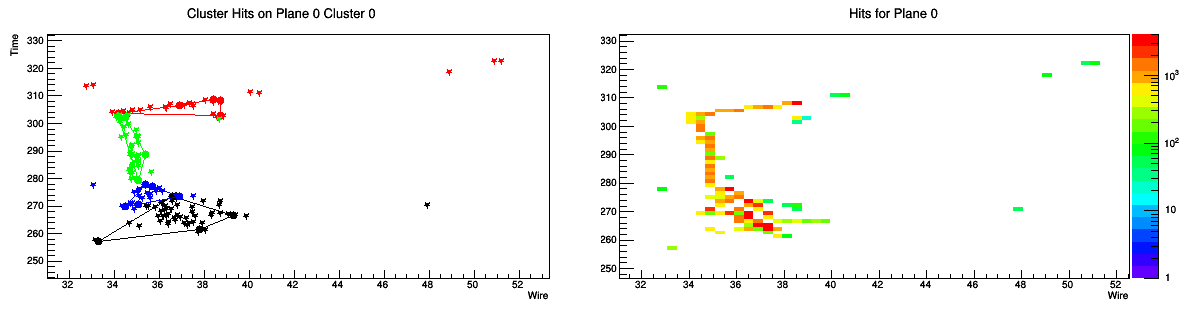
\includegraphics[width=150mm]{Figures/cluster_polygon_example.png}
\end{center}
\caption{\textit{Example of polygons associated with clusters in a BNB event. Left: hits are represented as stars. 
Hits belonging to different clusters are shown in different colors. Polygons associated with each cluster are shown as
bounding lines with the same color as the hits in that cluster. Right: event display showing the hits in this event
color-coded by the amount of charge in each hit.}}
\label{fig:cluster_polygon_example}
\end{figure}

\subsection{Polygon2D Class}
\paragraph{} A Polygon2D object is essentially an ordered list of 2D points that define the edges of a bounded surface
on a plane. The Polygon2D class has the following functionality:\newline
\newline
\textbf{Constructors}:\newline
Polygon2D(): creates a Polygon2D object with an empty list of edges.\newline
Polygon2D(std::vector\textless std::pair\textless float,float\textgreater \textgreater \&points): polygon edges assigned from input list.\newline
Polygon2D( Polygon2D \&poly1, Polygon2D \&poly2): returns intersection polygon.\newline
\textbf{Intrinsic Operations}\newline
float Area(): returns the area of the surface enclosed by the polygon\newline
float Perimeter(): returns the perimeter as measured by the sum-distance between consecutive edges.\newline
void UntanglePolygon(): Checks that the list of edges that defines the polygon is ordered correctly (no two lines cross)\newline
\textbf{External Comparisons}:\newline
bool PolyOverlap(const Polygon2D \&Poly2): determine if two polygons overlap in any way.\newline
bool PointInside(const std::pair\textless float,float\textgreater \&point): determine if a point is inside the polygon\newline
bool Contained(const Polygon2D \&poly2): determine if a polygon is fully contained within this polygon\newline


\subsection{Polygon Construction}
\paragraph{}To go from a list of hits in a cluster to a Polygon2D object we need to find a
way to determine the list of points that will define the boundary of the polygon.
\paragraph{}Polygons are created within the ClusterParams building-stage. This happens in \newline
RecoTool/ClusterRecoUtil/ClusterParamsAlg.cxx in the FillPolygon() function.
Within this function, the GeometryUtilities (LArUtil/GeometryUtilities.h) SelectPolygonHitList
function is called.
\paragraph{}Several steps are taken to construct a Polygon2D object that outlines a list of clusters in a hit.
This procedure can be seen in Fig.~\ref{fig:BoundingPolygon}.
\begin{figure}[h!]
\begin{center}
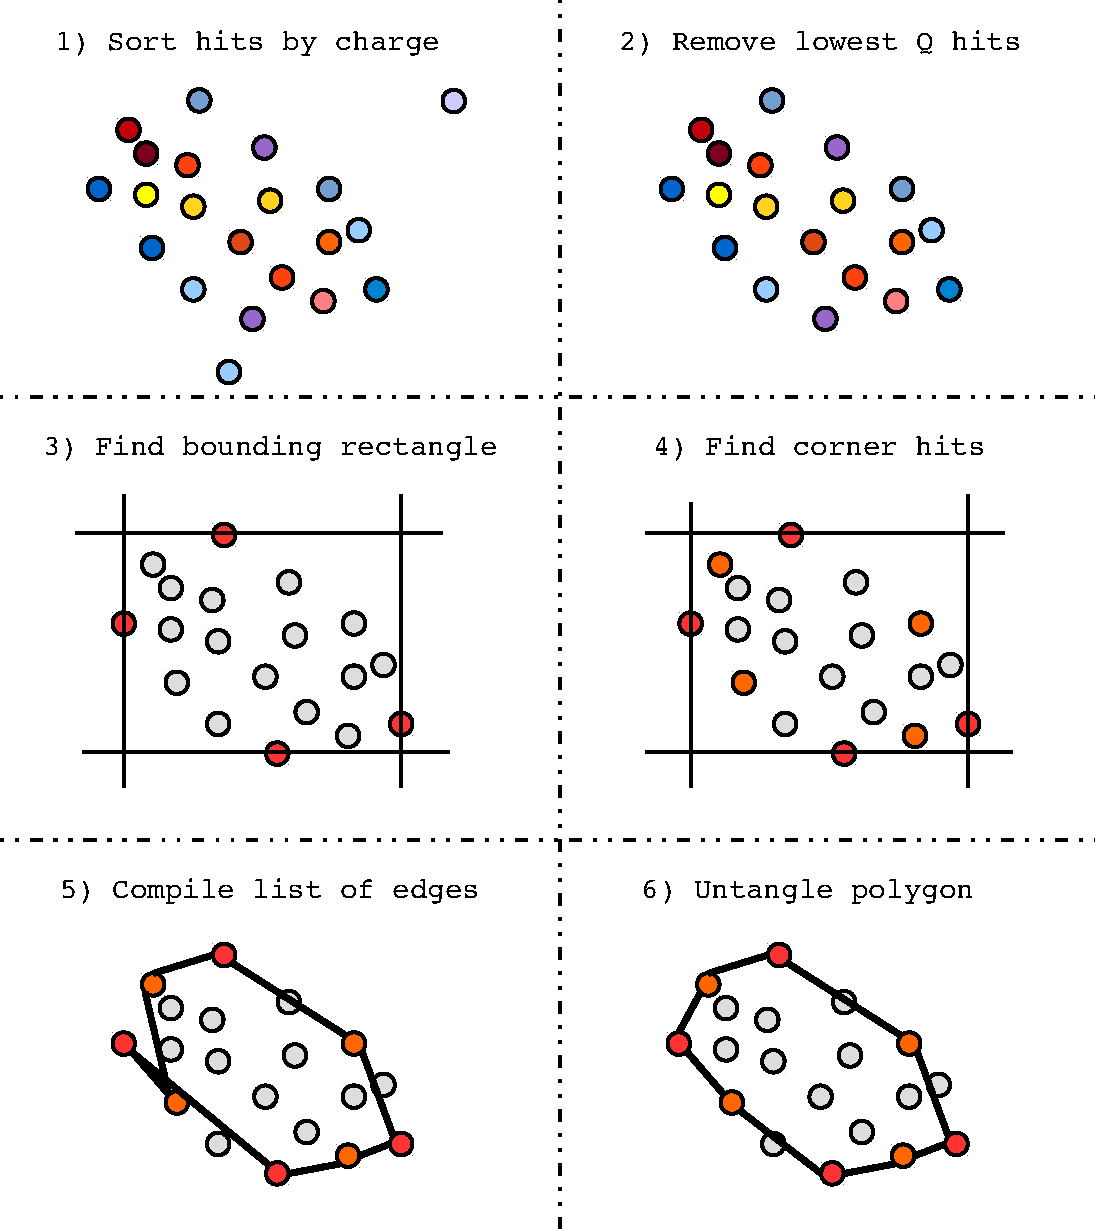
\includegraphics[width=140mm]{Figures/BoundingPolygon.pdf}
\end{center}
\caption{\textit{Procedure followed to create a Polygon2D associated to a cluster object}}
\label{fig:BoundingPolygon}
\end{figure}
\paragraph{}1) At first, a list of hits, ordered in decreasing hit charge, is created.
\paragraph{}2) subset list, containing all
the highest-charge hits whose total charge adds up to $\alpha$\% of the total cluster's charge is prepared. The 
default value of $\alpha$ used is 95. This step is taken to ensure we end up with a polygon that nicely matches
the cluster outline. We were of the idea that tt is better to exclude very low-amplitude hits if these would 
cause the polygon to grow too much in size and encompass large regions of empty area.
\paragraph{}3) Subsequently, the four hits that define an Axis-Aligned Bounded-Box which contains all sub-list hits
are identified. At this stage, we have (up to) four points defining a bounding rectangle.
\paragraph{}4) and 5) Next, we look for the hits closest to the corners of the rectangle. This gives us (up to) eight hits
representing the edges of a polygon.
\paragraph{}6) Finally, because a polygon is an ordered list of edges, we need to untangle the edges we found to make
sure the volume bounded by the polygon is well defined.

\end{document}

